\documentclass{article}
\usepackage{pgfplots}
\pgfplotsset{compat=1.18}
\usepackage{caption}

\begin{document}

\begin{figure}[h]
    \centering
    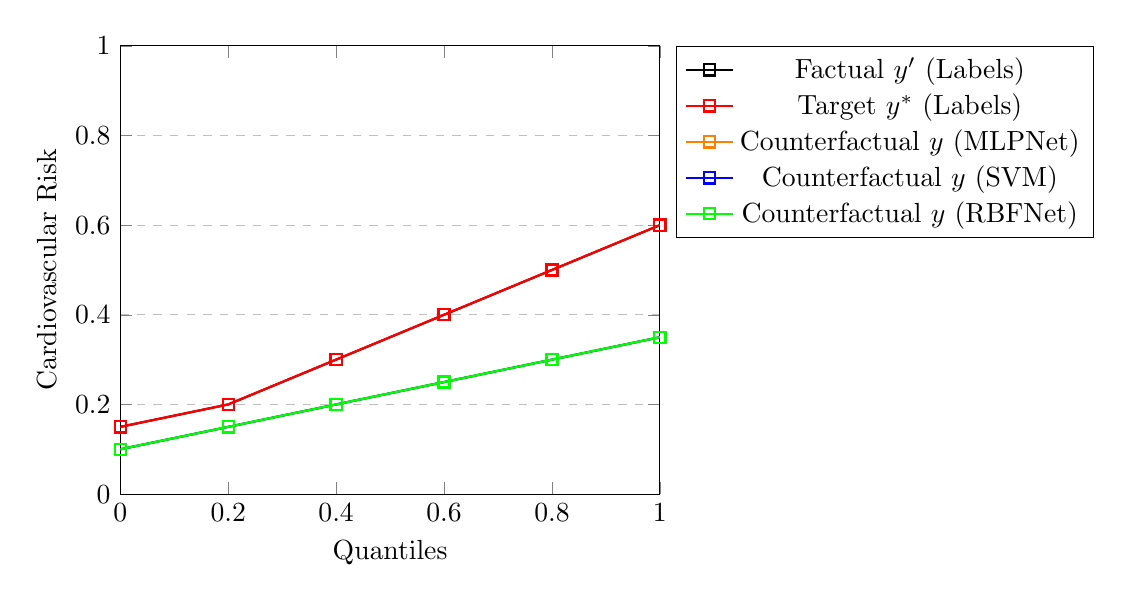
\begin{tikzpicture}
        \begin{axis}[
            xlabel={Quantiles},
            ylabel={Cardiovascular Risk},
            xmin=0, xmax=1,
            ymin=0, ymax=1,
            xtick={0,0.2,0.4,0.6,0.8,1},
            ytick={0,0.2,0.4,0.6,0.8,1},
            legend pos=outer north east,
            ymajorgrids=true,
            grid style=dashed,
        ]
        % Factual y' (Labels)
        \addplot[
            color=black,
            mark=square,
            thick,
        ] coordinates {
            (0, 0.15) (0.2, 0.2) (0.4, 0.3) (0.6, 0.4) (0.8, 0.5) (1, 0.6)
        };
        \addlegendentry{Factual $y'$ (Labels)}

        % Target y* (Labels)
        \addplot[
            color=red,
            mark=square,
            thick,
        ] coordinates {
            (0, 0.15) (0.2, 0.2) (0.4, 0.3) (0.6, 0.4) (0.8, 0.5) (1, 0.6)
        };
        \addlegendentry{Target $y^*$ (Labels)}

        % Counterfactual y (MLPNet)
        \addplot[
            color=orange,
            mark=square,
            thick,
        ] coordinates {
            (0, 0.1) (0.2, 0.15) (0.4, 0.2) (0.6, 0.25) (0.8, 0.3) (1, 0.35)
        };
        \addlegendentry{Counterfactual $y$ (MLPNet)}

        % Counterfactual y (SVM)
        \addplot[
            color=blue,
            mark=square,
            thick,
        ] coordinates {
            (0, 0.1) (0.2, 0.15) (0.4, 0.2) (0.6, 0.25) (0.8, 0.3) (1, 0.35)
        };
        \addlegendentry{Counterfactual $y$ (SVM)}

        % Counterfactual y (RBFNet)
        \addplot[
            color=green,
            mark=square,
            thick,
        ] coordinates {
            (0, 0.1) (0.2, 0.15) (0.4, 0.2) (0.6, 0.25) (0.8, 0.3) (1, 0.35)
        };
        \addlegendentry{Counterfactual $y$ (RBFNet)}
        \end{axis}
    \end{tikzpicture}
    \caption{The models are trained on all features whereas the \gls{dce} optimization is performed only on age, weight, and height.}
    \label{fig:dce_optimization}
\end{figure}

\end{document}